\documentclass[11pt]{article}

\usepackage[margin=1in]{geometry}
\usepackage{amsmath, amssymb, amsthm}
\usepackage{enumitem}
\usepackage{tikz}

\pagestyle{empty}

\begin{document}

\begin{center}
  {\Large\bfseries Weekly Assignment: Trees and Spanning Trees\\[4pt]
   (Epp~10.4, 10.5, \& 10.6)}
\end{center}

\bigskip

\noindent
Complete each of the following problems.  Show all work and justify your answers.

\bigskip

%% ─────────────────────────────────────────────
\noindent\textbf{Problem 1} (Epp 10.4 \#6). \;
If graphs are allowed to have an infinite number of vertices and
edges, then Lemma~10.4.1 is false.  Give a counterexample that
shows this.  In other words, give an example of an ``infinite
tree'' (a connected, circuit-free graph with an infinite number
of vertices and edges) that has no vertex of degree~1.

\bigskip

%% ─────────────────────────────────────────────
\noindent\textbf{Problem 2} (Epp 10.4 \#16). \;
Either draw a tree with twelve vertices and fifteen edges,
or explain why no such graph exists.

\bigskip

%% ─────────────────────────────────────────────
\noindent\textbf{Problem 3} (Epp 10.4 \#17). \;
Either draw a graph with six vertices and five edges that is
\emph{not} a tree, or explain why no such graph exists.

\bigskip

%% ─────────────────────────────────────────────
\noindent\textbf{Problem 4} (Epp 10.5 \#12). \;
Either draw a full binary tree with eight internal vertices and
seven leaves, or explain why no such graph exists.

\bigskip

%% ─────────────────────────────────────────────
\noindent\textbf{Problem 5} (Epp 10.5 \#14). \;
Either draw a full binary tree with seven vertices,
or explain why no such graph exists.

\bigskip

%% ─────────────────────────────────────────────
\noindent\textbf{Problem 6} (Epp 10.6 \#10). \;
For the weighted graph below, find all minimum spanning trees
that can be obtained using
\begin{enumerate}[label=\textbf{(\alph*)}]
  \item Kruskal's algorithm, and
  \item Prim's algorithm starting with vertex~$t$.
\end{enumerate}
Indicate the order in which edges are added to form each tree.

\begin{center}
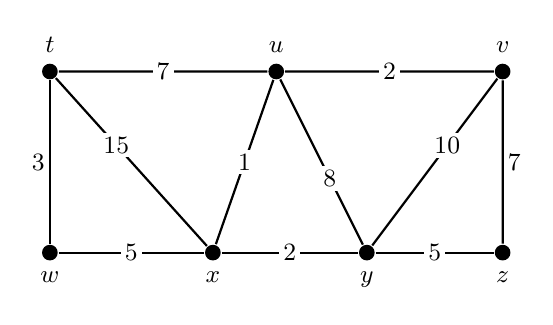
\begin{tikzpicture}[
    vertex/.style={circle, fill=black, inner sep=2pt},
    every node/.style={font=\small},
    wt/.style={fill=white, inner sep=1.5pt, font=\small},
    thick,
    scale=1.15
  ]
  % Top row
  \node[vertex, label=above:$t$] (t) at (0,2)   {};
  \node[vertex, label=above:$u$] (u) at (2.5,2) {};
  \node[vertex, label=above:$v$] (v) at (5,2)   {};
  % Bottom row
  \node[vertex, label=below:$w$] (w) at (0,0)   {};
  \node[vertex, label=below:$x$] (x) at (1.8,0) {};
  \node[vertex, label=below:$y$] (y) at (3.5,0) {};
  \node[vertex, label=below:$z$] (z) at (5,0)   {};

  % Top edges
  \draw (t) -- node[wt] {7}  (u);
  \draw (u) -- node[wt] {2}  (v);
  % Side edges
  \draw (t) -- node[wt,left] {3}  (w);
  \draw (v) -- node[wt,right] {7} (z);
  % Bottom edges
  \draw (w) -- node[wt] {5}  (x);
  \draw (x) -- node[wt] {2}  (y);
  \draw (y) -- node[wt] {5}  (z);
  % Diagonals / inner edges
  \draw (t) -- node[wt,pos=0.4] {15} (x);
  \draw (u) -- node[wt] {1}  (x);
  \draw (u) -- node[wt,pos=0.6] {8}  (y);
  \draw (v) -- node[wt,pos=0.4] {10} (y);
\end{tikzpicture}
\end{center}

\bigskip

%% ─────────────────────────────────────────────
\noindent\textbf{Problem 7} (Proof). \;
Let $G$ be a connected graph.  Prove that an edge~$e$ is contained
in every spanning tree of~$G$ if and only if removing~$e$
disconnects~$G$.

\medskip\noindent
\emph{Hint}: This is a biconditional, so prove both directions.
For the forward direction, consider what happens if removing~$e$
does \emph{not} disconnect~$G$.  For the converse, suppose~$e$ is
\emph{not} in some spanning tree~$T$ and think about what $T$
tells you about the connectivity of~$G-e$.

\end{document}
